\documentclass[10pt,a4paper]{article}

\usepackage[a4paper,top=0.95cm,bottom=0.95cm,left=1.15cm,right=1.15cm]{geometry}
\usepackage{fontspec}
\usepackage[french]{babel}
\usepackage[hidelinks]{hyperref}
\usepackage{xcolor}
\usepackage{graphicx}
\usepackage{titlesec}
\usepackage{enumitem}

\setmainfont{Arial}
\pagestyle{empty}
\setlength{\parindent}{0pt}
\setlength{\parskip}{0pt}
\linespread{0.98}
\setlist[itemize]{leftmargin=1.05em,itemsep=0pt,topsep=1pt,parsep=0pt}

\definecolor{heading}{HTML}{123867}
\titleformat{\section}{\large\bfseries\color{heading}}{}{0pt}{}[\vspace{-6pt}\rule{\linewidth}{0.5pt}]
\titlespacing{\section}{0pt}{5pt}{3pt}

\newif\ifwithphoto
\withphotofalse
\IfFileExists{with_photo.flag}{\withphototrue}{}

\newcommand{\role}[3]{%
  \textbf{#1} \hfill #3\\
  \textit{#2}\vspace{1pt}
}

\newcommand{\edu}[4]{%
  \textbf{#1} -- #2 \hfill #3 #4\\[-1pt]
}

\begin{document}

\ifwithphoto
\begin{minipage}[c]{0.76\linewidth}
{\LARGE \textbf{Kossi Richard Allado}}\\
\textbf{Etudiant ingenieur en informatique | Reseaux, systemes, securite et support IT}\\
Beni Mellal, Maroc | +212 621 074 305 | \href{mailto:alladokossirichard2025@gmail.com}{alladokossirichard2025@gmail.com}\\
\href{https://allakori.github.io/}{allakori.github.io} | \href{https://github.com/ALLAKORI}{github.com/ALLAKORI} | \href{https://www.linkedin.com/in/kossi-richard-allado-50177b2a5}{linkedin.com/in/kossi-richard-allado}
\end{minipage}
\hfill
\begin{minipage}[c]{0.18\linewidth}
\raggedleft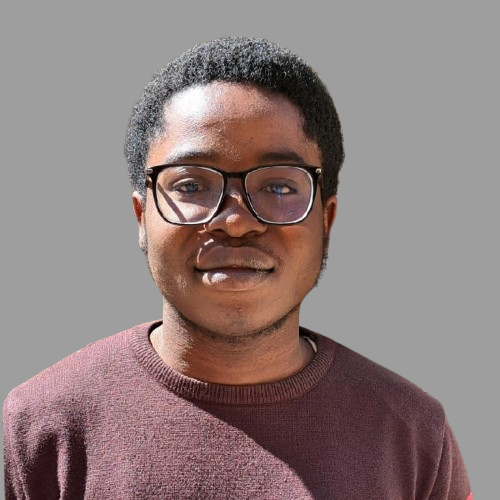
\includegraphics[width=2.35cm]{photo_richard.png}
\end{minipage}
\else
{\LARGE \textbf{Kossi Richard Allado}}\\
\textbf{Etudiant ingenieur en informatique | Reseaux, systemes, securite et support IT}\\
Beni Mellal, Maroc | +212 621 074 305 | \href{mailto:alladokossirichard2025@gmail.com}{alladokossirichard2025@gmail.com}\\
\href{https://allakori.github.io/}{allakori.github.io} | \href{https://github.com/ALLAKORI}{github.com/ALLAKORI} | \href{https://www.linkedin.com/in/kossi-richard-allado-50177b2a5}{linkedin.com/in/kossi-richard-allado}
\fi

\section{Profil}
Etudiant ingenieur en cybersecurite et intelligence artificielle a l'ENSA Beni Mellal, interesse par les reseaux, les systemes, la securite informatique et le support technique. Pratique de Linux, Nmap, Wireshark, SSH, analyse de logs, hardening, securite applicative et documentation technique. Recherche un stage en reseaux/securite pour contribuer a des missions de support, maintenance, diagnostic reseau, administration systemes ou securisation d'environnements informatiques.

\section{Competences techniques}
\textbf{Reseaux / diagnostic :} Nmap, Wireshark, SSH, analyse de trafic, enumeration, diagnostic reseau.\\
\textbf{Systemes / securite :} Linux, Windows logs, hardening Linux, SELinux, AppArmor, Lynis, auditd.\\
\textbf{Securite applicative :} bases web, SQL injection, XSS, Burp Suite, DVWA, bonnes pratiques de correction.\\
\textbf{Support / automatisation :} troubleshooting, analyse d'incidents, Bash, Python, SQL, Git/GitHub, rapports.

\section{Projets techniques}
\textbf{Plateforme IAM, PKI et securite applicative} \hfill Reseaux / securite\\
\href{https://github.com/ALLAKORI/cybersecurity-iam-labs}{github.com/ALLAKORI/cybersecurity-iam-labs}
\begin{itemize}
  \item Deploiement d'un environnement IAM avec Keycloak : utilisateurs, roles, MFA/TOTP, RBAC et tests d'acces.
  \item Mise en pratique OpenSSL/PKI et tests applicatifs, avec analyse des risques et propositions de correction.
\end{itemize}

\textbf{Investigation de logs et reponse a incident} \hfill Logs / detection\\
\href{https://allakori.github.io/writeups/tryhackme/volt-typhoon/}{Write-up technique}
\begin{itemize}
  \item Analyse de logs Windows et applicatifs avec Splunk pour reconstruire une attaque et identifier les evenements importants.
  \item Production d'une timeline, extraction d'indicateurs et redaction d'un rapport technique exploitable.
\end{itemize}

\textbf{Analyse forensic disque et memoire pour reponse a incident} \hfill Systemes / DFIR\\
\href{https://github.com/ALLAKORI/linux-security-labs}{github.com/ALLAKORI/linux-security-labs}
\begin{itemize}
  \item Analyse d'artefacts systeme avec WinPMEM, Volatility, Autopsy et FTK Imager.
  \item Identification de processus, connexions reseau, traces utilisateur et elements utiles a la remediation.
\end{itemize}

\section{Experience}
\role{Stagiaire IA / Maintenance predictive}{ONEE - Branche Eau, Kasba Tadla}{Aout 2025}
\begin{itemize}
  \item Preparation et analyse de donnees capteurs pour predire des defauts de pompes haute pression.
  \item Entrainement d'un modele Random Forest avec Python, Pandas et Scikit-learn.
  \item Creation d'une interface Tkinter pour tester les predictions et valider le prototype.
\end{itemize}

\section{Formation}
\edu{Cycle ingenieur}{Cybersecurite et Intelligence Artificielle, ENSA Beni Mellal}{2024 - Present}{}
\edu{DEUST}{Mathematiques, Informatique, Physique, FST Fes}{2022 - 2024}{-- Mention Bien}
\edu{Baccalaureat scientifique}{Serie D, Lycee de Djagble, Togo}{2022}{-- Mention Tres Bien}

\section{Certifications et realisations}
Cisco Ethical Hacker | Google Cybersecurity : Foundations et Play It Safe | TryHackMe Junior Penetration Tester Learning Path | TryHackMe Advent of Cyber 2025 | Udemy Cryptography and Hashing | 1ere place CSIA CTF 2026 avec Team GHOSTSHELL

\section{Langues}
Francais : courant | Anglais : professionnel technique | Ewe : langue maternelle

\end{document}
